\documentclass[a4paper,12pt]{article}

\usepackage[T2A]{fontenc}
\usepackage[utf8x]{inputenc}
\usepackage[russian,english]{babel}
\usepackage{amssymb,amsfonts,amsmath,cite,enumerate,float,indentfirst}
\usepackage{graphicx}
\usepackage{color}
\usepackage{xcolor}
\usepackage{fancyhdr}

\usepackage{array}
\usepackage{supertabular}
\usepackage{hhline}
\usepackage{semantic}


\usepackage{listings}
\lstloadlanguages{c++,c,tex,bash,sql,pascal,html}
\lstset{
	language=c,inputencoding=utf8x,
	extendedchars=\true,captionpos=b,tabsize=4,
	frame=lines,
	keywordstyle=\color{blue},commentstyle=\color{green},stringstyle=\color{red},
	breaklines=true,showstringspaces=false,basicstyle=\footnotesize
}
\lstset{
	language=tex,inputencoding=utf8x,
	extendedchars=\true,captionpos=b,tabsize=4,
	frame=lines,
	keywordstyle=\color{blue},commentstyle=\color{green},stringstyle=\color{red},
	breaklines=true,showstringspaces=false,basicstyle=\footnotesize
}
\lstset{
	language=html,inputencoding=utf8x,
	extendedchars=\true,captionpos=b,tabsize=4,
	frame=lines,
	keywordstyle=\color{blue},commentstyle=\color{green},stringstyle=\color{red},
	breaklines=true,showstringspaces=false,basicstyle=\footnotesize
}
\lstset{
	language=c++,inputencoding=utf8x,
	extendedchars=\true,captionpos=b,tabsize=4,
	frame=lines,
	keywordstyle=\color{blue},commentstyle=\color{green},stringstyle=\color{red},
	breaklines=true,showstringspaces=false,basicstyle=\footnotesize
}
\lstset{
	language=sql,inputencoding=utf8x,
	extendedchars=\true,captionpos=b,tabsize=4,
	frame=lines,
	keywordstyle=\color{blue},commentstyle=\color{green},stringstyle=\color{red},
	breaklines=true,showstringspaces=false,basicstyle=\footnotesize
}
\lstset{
	language=pascal,inputencoding=utf8x,
	extendedchars=\true,captionpos=b,tabsize=4,
	frame=lines,
	keywordstyle=\color{blue},commentstyle=\color{green},stringstyle=\color{red},
	breaklines=true,showstringspaces=false,basicstyle=\footnotesize
}

\usepackage{geometry} % Меняем поля страницы
\geometry{left=2cm}% левое поле
\geometry{right=1.5cm}% правое поле
\geometry{top=1cm}% верхнее поле
\geometry{bottom=2cm}% нижнее поле

\renewcommand{\theenumi}{\arabic{enumi}}
\renewcommand{\labelenumi}{\arabic{enumi}}
\renewcommand{\theenumii}{.\arabic{enumii}}
\renewcommand{\labelenumii}{\arabic{enumi}.\arabic{enumii}.}
\renewcommand{\theenumiii}{.\arabic{enumiii}}
\renewcommand{\labelenumiii}{\arabic{enumi}.\arabic{enumii}.\arabic{enumiii}.}


\begin{document}

\begin{titlepage}
\newpage

\begin{center}
Федеральное агентство по образованию РФ\\
Пермский Национальный Исследовательский Политехнический Университет\\
Кафедра Информационных Технологий и Автоматизированных Систем
\end{center}

\vspace{8em}

\begin{center}
\Large Кузнецов Д.Б., Вагин Д.А.
\end{center}

\vspace{2em}

\begin{center}
\Huge \textbf{Теория языков программирования и методы трансляции}
\end{center}
\begin{center}
Методические указания по выполниению лабораторных работ\\
для специальности ПОВТ
\end{center}

\vspace{\fill}

\begin{center}
г. Пермь 2011
\end{center}

\end{titlepage}

\newpage
\section{Введение}
Предлагаемый лабораторный практикум предназначен для  приобретение знаний и навыков в области использования и разработки как трансляторов в целом, так и отдельных элементов — лексического, синтаксического и семантического анализаторов, генератора выходного кода. 

\subsection{Требования к аппаратному обеспечению}

\paragraph{Вариант 1: Выполненние работ на локальном компьютере}
Компьютер должен обеспечивать возможность запуска операционной системы, текстового редактора, и средств компиляции исходного кода. Необходимо иметь 200МБ свободного места на жёстком диске для установки необходимого по и хранения исходных текстов программ.

\paragraph{Вариант 2: Выполненние работ на удалённом сервере}
Сервер должен иметь технические характеристики достаточные для запуска операционной системы и сервисов для удалённого подключения. Более точные аппартные характеристики зависят от версии ядра и системных библиотек. Для запуска последних версий без графического режима вполне достаточно процессор с частотой от 300 МГц, ОЗУ от 512 МБ, свободно дисковое пространство от 500 МБ. Локальное рабочее место должно быть оборудовано терминалом, подключенным к серверу.

\subsection{Требования к системному программному обеспечению}
Рассмариваемое ниже системное программное обеспечение должно быть установлено на локальном компьютере (Вариант 1 аппаратного обеспечения) или на сервере (Вариант 2 аппаратного обеспечения).
\paragraph{}
Для выполнения лабораторных работ потребуется инструментарий для сборки компиляции программ на языке С — GNU gcc, а так же консольные программы yacc и lex.

\newpage
\section{Лабораторная работа №1\\
	Построение лексического анализатора на основании автоматной грамматики}
\subsection{Цель}
\begin{itemize}
	\item Научитсья строить лексические анализаторы на основе автоматной грамматики
\end{itemize}

\subsection{Порядок выполнения}
\begin{enumerate}
	\item Построить автоматную грамматику
	\item Построить автомат
	\item Привести к детерминированному автомату
	\item Реализовать автомат программно на языке программирования C
	\item Написать отчет
\end{enumerate}

\subsection{Рекомендации по выполнению}
\begin{itemize}
	\item Используйте массивы фиксированной длины
	\item Задавайте данные внутри исходного кода
\end{itemize}

\subsection{Состав отчета}
\begin{itemize}
	\item Титульный лист (фамилия, группа, номер варианта, наименование работы, задание)
	\item Текст задания
	\item Грамматика
	\item Диаграмма переходов
	\item Автоматы
	\item Текст программы
\end{itemize}

\subsection{Варианты заданий}
В задании указано содержательное описание грамматики и простейший пример для облегчения понимания.
\begin{enumerate}
	\item Одинаковые символы стоят парами: $aabbaabbbbaa$
	\item В начале строки $a$: $ababbbabb$
	\item Первый символ — не важен, далее одни $a$: $baaaaaaaaa$, $aaaaaaaaaa$
	\item Либо одни $a$, либо одни $b$: $aaaaaaaaaa$, $bbbbbbbbb$
	\item В конце строки $b$: $ababbbabb$
	\item Одинаковые символы не должны стоять рядом: $ababababab$, $bababababa$
	\item В строке должна встретиться хотя бы одна буква $a$: $bbbbbabbb$, $aaaaaaaa$
	\item Предпоследним символом строки должна быть $b$, $abbabaabb$
	\item Вторым символом строки должна быть $a$: $baaaaabbb$
	\item Два последних символа должны быть $b$: $abababb$, $bbbbbb$
	\item Первый и третий символы должны быть разными: $aabbbabab$, $baaabbbab$
	\item Первый и последний символы должны быть одинковыми: $ababababa$, $babbbabab$
\end{enumerate}

\subsection{Пример}
\paragraph{Задание}
Символы $a$ и $b$ стоят парами: abbaabab, baabbaba.
\paragraph{Грамматика}
Построим грамматику по заданию: \\
$S -> aB$\\
$S -> bA$\\
$B -> bF$\\
$A -> aF$\\
$B -> bS$\\
$A -> aS$\\
$F -> \dashv$

\paragraph{}\vspace{1em}
Диаграмма переходов\\

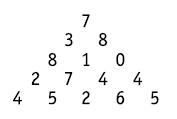
\includegraphics[scale=0.5]{lab1/images/image1.jpg}\vspace{1em}
%% TODO: сделать диаграмму на latex'е

\begin{tabular}[l]{c|cccc}
    & $-$ & $-$   & $-$   & $+$ \\
\hline
    & $S$ & $A$   & $B$   & $F$ \\
$a$ & $B$ & $S,F$ &       &     \\
$b$ & $A$ &       & $S,F$ &     \\
\end{tabular}

\paragraph{}
Детерминированный автомат\\

\begin{tabular}[l]{c|cccccc}
    & $-$ & $-$       & $-$       & $+$    & $-$    & $+$       \\
\hline
    & $S$ & $A$       & $B$       & $F$    & $\{\}$ & $\{S,F\}$ \\
$a$ & $B$ & $\{S,F\}$ &  $\{\}$   & $\{\}$ & $\{\}$ & $B$       \\
$b$ & $A$ & $\{\}$    & $\{S,F\}$ & $\{\}$ & $\{\}$ & $A$       \\
\end{tabular}

\paragraph{Программа}
Напишем программу на языке программирования C. Откомпилировать её можно компилятором GNU gcc так: \emph{gcc -o program lab1.c}

\begin{lstlisting}[language=c,{caption=анализатор}]
#include <stdio.h>

#define S  0 /* S */
#define A  1 /* A */
#define B  2 /* B */
#define F  3 /* F */
#define H  4 /* {S,F} */
#define W  5 /* {} */

#define P  1 /* + */
#define M  0 /* - */

#define a 0 /* a */
#define b 1 /* b */

struct action
{
	int sos; /* состояние */
	int out; /* вывод */
};

int main()
{
	int table[2][6];
	table[a][S] = B;
	table[b][S] = A;
	table[a][A] = H;
	table[b][A] = W;
	table[a][B] = W;
	table[b][B] = H;
	table[a][F] = W;
	table[b][F] = W;
	table[a][W] = W;
	table[b][W] = W;
	table[a][H] = B;
	table[b][H] = A;

	int output[6];
	output[S] = M;
	output[A] = M;
	output[B] = M;
	output[F] = P;
	output[W] = M;
	output[H] = P;


	int input[]={b,a,a,b};
	int n = 4, i;
	int isos = S;
 
	for( i=0; i<n; ++i)
	{
		isos=table[input[i]][isos];
	}

	printf("%d\n", output[isos]);
	return 0;
}
\end{lstlisting}


\newpage
\section{Лабораторная работа №2\\
	Построение лексического анализатора с использованием lex}

\subsection{Цели}
\begin{itemize}
	\item Познакомиться с «регулярными выражениями»
	\item Познакомиться с программой lex
	\item Научиться строить лексические анализаторы с использованием lex
\end{itemize}

\subsection{Порядок выполнения}
\begin{enumerate}
	\item Построить регулярное выражение
	\item Составить файл для lex
	\item Получить программу на Си
	\item Откомпилировать и запустить
	\item Написать отчет
\end{enumerate}

\subsection{Состав отчёта}
\begin{itemize}
	\item Титульный лист (фамилия, группа, номер варианта, наименование работы, задание)
	\item Текст задания
	\item Текст программы на lex
	\item Результаты работы программы
\end{itemize}

\subsection{Варианты заданий}
В задании указано содержательное описание грамматики и простейший пример для облегчения понимания.
\begin{enumerate}
	\item Одинаковые символы стоят парами: $aabbaabbbbaa$
	\item В начале строки $a$: $ababbbabb$
	\item Первый символ — не важен, далее одни $a$: $baaaaaaaaa$, $aaaaaaaaaa$
	\item Либо одни $a$, либо одни $b$: $aaaaaaaaaa$, $bbbbbbbbb$
	\item В конце строки $b$: $ababbbabb$
	\item Одинаковые символы не должны стоять рядом: $ababababab$, $bababababa$
	\item В строке должна встретиться хотя бы одна буква $a$: $bbbbbabbb$, $aaaaaaaaa$
	\item Предпоследним символом строки должна быть $b$, $abbabaabb$
	\item Вторым символом строки должна быть $a$: $baaaaabbb$
	\item Два последних символа должны быть $b$: $abababb$, $bbbbbb$
	\item Первый и третий символы должны быть разными: $aabbbabab$, $baaabbbab$
	\item Первый и последний символы должны быть одинковыми: $ababababa$, $babbbabab$
\end{enumerate}

\subsection{Пример}
\paragraph{Задание}
Символы $a$ и $b$ стоят парами: $abbaabab$, $baabbaba$.

\paragraph{Регулярное выражение}
Регулярное выражение будет иметь вид: (ab|ba)+

\paragraph{Программа на lex}
Создадим файл lab3.l со следующим содержимым:

\begin{lstlisting}[language=c,{caption=lab3.l}]
%%
(ab|ba)+ { printf("Yes");}
.* { printf("No"); }
%%

yyerror(char *str)
{ printf(str); }

main()
{ yylex(); }
\end{lstlisting}

\paragraph{}
Программу на C получим простой командой. lab3.c - имя выходного файла, lab3.l имя входного файла на lex.

\begin{verbatim}
flex -o lab3.c lab3.l
\end{verbatim}

\paragraph{}
Для компиляции воспользуемся компилятором gcc.
\begin{verbatim}
gcc -o lab3 lab3.c -lfl
\end{verbatim}

Запуск осуществляется так:
\begin{verbatim}
./lab3
ababbababa
Yes

bbbaa
No	
\end{verbatim}

\newpage

\section{Лабораторная работа №3\\
	Построение синтаксического анализатора на основании LL(1) грамматики}

\subsection{Порядок выполнения}
\begin{enumerate}
	\item Построить LL(1) грамматику
	\item Определить множества выбора для каждого правила
	\item Изобразить низходящую схему разбора
	\item Разработать лексический анализатор на базе lex
	\item Построить МП-автомат по грамматике
	\item Реализовать МП-автомат
	\item Реализовать синтаксический анализ методом рекурсивного спуска	
\end{enumerate}

\subsection{Варианты заданий}
В задании указано содержательное описание грамматики и простейший пример для облегчения понимания.
\begin{enumerate}
	\item конструкция for языка с++. 
\begin{lstlisting}[language=c++,{caption=for}]
for(
	a=0, b=76; 
	i<10 && b>0 ;
	++i, b=i+1
){ 
	b++;
	i++;
}
\end{lstlisting}

	\item конструкция if языка c++. 
\begin{lstlisting}[language=c++,{caption=if}]
if(a==0 && b<=0)
{
	a=b; b++;
}
else
{
	a++; 
	b+=2;
}
\end{lstlisting}

	\item конструкция switch языка c++. 
\begin{lstlisting}[language=c++,{caption=switch}]
switch(a){ 
	case 1: a=1; 
	case 3: 
	case 2: a++; break; 
	default: a=0;
}
\end{lstlisting}

	\item тэг img языка разметки HTML: 
\begin{lstlisting}[language=html,{caption=img}]
<img src="/images/a.png" width="20" height="30" 
	alt="картинка" />
\end{lstlisting}

	\item Объявление функции в c++:
\begin{lstlisting}[language=c++,{caption=func}]
int funcname(int a, char b, float c = 0.1);
\end{lstlisting}

	\item тэг table языка разметки HTML: 
\begin{lstlisting}[language=html,{caption=table}]
<table>
	<tr>
		<th>заголовок 1</th>
		<th>заголовок 2</th>
	</tr>
	<tr>
		<td>ячейка 1</td>
		<td>ячейка 2</td>
	</tr>
	<tr>
		<td>ячейка 3</td>
		<td>ячейка 4</td>
	</tr>
</table>
\end{lstlisting}

	\item тэг ul (ненумерованный список) языка разметки HTML: 
\begin{lstlisting}[language=html,{caption=ul}]
<ul>
	<li>item 1</li>
	<li>item 2</li>
	<li>item 3</li>
</ul>
\end{lstlisting}

	\item конструкция while языка c++. 
\begin{lstlisting}[language=c++,{caption=while}]
while( a>0 || b<76){
	b++;
	a++;
}
\end{lstlisting}

	\item конструкция do-while языка c++. 
\begin{lstlisting}[language=c++,{caption=do-while}]
do{
	b++;
	a++;
}while( a>0 || b<76);
\end{lstlisting}

	\item конструкция insert языка запросов SQL:
\begin{lstlisting}[language=sql,{caption=insert}]
insert into tablename(pk,column1,column2) 
values (1, 2 , 'varchar');
\end{lstlisting}

	\item конструкция select языка запросов SQL:
\begin{lstlisting}[language=sql,{caption=select}]
select pk, column1, column2
from tablename
where column1 = 2 
	and column2 like 'xxx%';
\end{lstlisting}

	\item конструкция delete языка запросов SQL:
\begin{lstlisting}[language=sql,{caption=delete}]
delete from tablename
where column1 = 1
	or column2 like 'xxx%';
\end{lstlisting}

	\item тэг form языка разметки HTML: 
\begin{lstlisting}[language=html,{caption=form}]
<form methid="post" action="/registration/">
	<input type="text" name="login" />
	<input type="text" name="email" />
	<input type="password" name="password" />
	<input type="submit"/>
</form>
\end{lstlisting}

	\item конструкция if языка Pascal: 
\begin{lstlisting}[language=pascal,{caption=if}]
if (a <= 10) or (b >= 2) then
begin
	a := 10;
	b := 10;
end else
	a := b;

\end{lstlisting}

	\item конструкция for языка Pascal: 
\begin{lstlisting}[language=pascal,{caption=for}]
for i:= 0 to 10 step 2 do 
begin
	a := i;
end;
\end{lstlisting}

\end{enumerate}

\subsection{Пример реализации}
\begin{itemize}
	\item Пример МП автомата: http://www.softcraft.ru/translat/lect/t07-07.shtml
	\item Пример программы с использованием рекурсивного спуска: http://www.softcraft.ru/translat/lect/t07-08.shtml
\end{itemize}

\newpage
\section{Лабораторная работа №4\\
	Построение синтаксического анализатора на основании LR грамматики}

\subsection{Порядок выполнения}
\begin{enumerate}
	\item Построить грамматику с предшествованием
	\item Определить отношения предшествования
	\item Изобразить восходящую схему разбора
	\item Выполнить свертку заданного примера
	\item Разработать синтаксический анализатор на базе yacc
	\item Разработать лексический анализатор на базе lex
	\item Выполнить синтаксический анализ заданного примера
\end{enumerate}

\subsection{Варианты заданий}
В задании указано содержательное описание грамматики и простейший пример для облегчения понимания.
\begin{enumerate}
	\item конструкция for языка с++. 
\begin{lstlisting}[language=c++,{caption=for}]
for(
	a=0, b=76; 
	i<10 && b>0 ;
	++i, b=i+1
){ 
	b++;
	i++;
}
\end{lstlisting}

	\item конструкция if языка c++. 
\begin{lstlisting}[language=c++,{caption=if}]
if(a==0 && b<=0)
{
	a=b; b++;
}
else
{
	a++; 
	b+=2;
}
\end{lstlisting}

	\item конструкция switch языка c++. 
\begin{lstlisting}[language=c++,{caption=switch}]
switch(a){ 
	case 1: a=1; 
	case 3: 
	case 2: a++; break; 
	default: a=0;
}
\end{lstlisting}

	\item тэг img языка разметки HTML: 
\begin{lstlisting}[language=html,{caption=img}]
<img src="/images/a.png" width="20" height="30" 
	alt="картинка" />
\end{lstlisting}

	\item Объявление функции в c++:
\begin{lstlisting}[language=c++,{caption=func}]
int funcname(int a, char b, float c = 0.1);
\end{lstlisting}

	\item тэг table языка разметки HTML: 
\begin{lstlisting}[language=html,{caption=table}]
<table>
	<tr>
		<th>заголовок 1</th>
		<th>заголовок 2</th>
	</tr>
	<tr>
		<td>ячейка 1</td>
		<td>ячейка 2</td>
	</tr>
	<tr>
		<td>ячейка 3</td>
		<td>ячейка 4</td>
	</tr>
</table>
\end{lstlisting}

	\item тэг ul (ненумерованный список) языка разметки HTML: 
\begin{lstlisting}[language=html,{caption=ul}]
<ul>
	<li>item 1</li>
	<li>item 2</li>
	<li>item 3</li>
</ul>
\end{lstlisting}

\item конструкция while языка c++. 
\begin{lstlisting}[language=c++,{caption=while}]
while( a>0 || b<76){
	b++;
	a++;
}
\end{lstlisting}

\item конструкция do-while языка c++. 
\begin{lstlisting}[language=c++,{caption=do-while}]
do{
	b++;
	a++;
}while( a>0 || b<76);
\end{lstlisting}

	\item конструкция insert языка запросов SQL:
\begin{lstlisting}[language=sql,{caption=insert}]
insert into tablename(pk,column1,column2) 
values (1, 2 , 'varchar');
\end{lstlisting}

	\item конструкция select языка запросов SQL:
\begin{lstlisting}[language=sql,{caption=select}]
select pk, column1, column2
from tablename
where column1 = 2 
	and column2 like 'xxx%';
\end{lstlisting}

	\item конструкция delete языка запросов SQL:
\begin{lstlisting}[language=sql,{caption=delete}]
delete from tablename
where column1 = 1
	or column2 like 'xxx%';
\end{lstlisting}

	\item тэг form языка разметки HTML: 
\begin{lstlisting}[language=html,{caption=form}]
<form methid="post" action="/registration/">
	<input type="text" name="login" />
	<input type="text" name="email" />
	<input type="password" name="password" />
	<input type="submit"/>
</form>
\end{lstlisting}

	\item конструкция if языка Pascal: 
\begin{lstlisting}[language=pascal,{caption=if}]
if (a <= 10) or (b >= 2) then
begin
	a := 10;
	b := 10;
end else
	a := b;

\end{lstlisting}

	\item конструкция for языка Pascal: 
\begin{lstlisting}[language=pascal,{caption=for}]
for i:= 0 to 10 step 2 do 
begin
	a := i;
end;
\end{lstlisting}

\end{enumerate}

\subsection{Пример реализации}
Построим грамматику \\
$S -> sXfX$\\
$X -> xY$\\
$X -> x$\\
$Y -> ,xY$\\
$Y -> ,x$\\

\begin{tabular}[l]{c|cccccc}
    & $s$ & $X$ & $Y$ & $x$ & $f$ & $,$ \\
\hline
$s$ &     & $=$ &     & $<$ &     &     \\
$X$ &     &     &     &     & $=$ &     \\
$Y$ &     &     &     &     & $>$ &     \\
$x$ &     &     & $=$ &     & $>$ & $<$ \\
$f$ &     & $=$ &     & $<$ &     &     \\
$,$ &     &     &     & $=$ &     &     \\
\end{tabular}

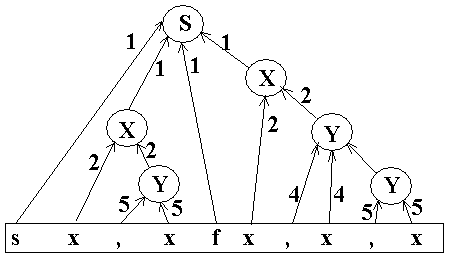
\includegraphics[scale=1.0]{lab4/lab4.png}\vspace{1em}

Обозначим условно \textasciicircum как начало, а \$ как конец строки.

\begin{math}
sx,xfx => \\
<s<x<, \doteq x>f<x> => \\
<s<x \doteq Y>f \doteq X> => \\
<s<X \doteq f \doteq >X> => <S>
\end{math}\\

\begin{lstlisting}[language=tex,{caption=lab4.l}]
%%
x               { return x; }
f               { return f; }
,               { return comma; }
.               { return yytext; }
%%
\end{lstlisting}

\begin{lstlisting}[language=tex,{caption=lab4.y}]
%start start

%token f x comma

%%

start:  X f X { printf("%s\n", "OK");}
        ;
X :     x
        | x Y
        ;
Y :     comma x
        | comma x Y
        ;

%%
/* start of programs */
#include "lex.yy.c"

main() { return  yyparse();}

yyerror(char *s) { fprintf(stderr,"%s\n",s); }
\end{lstlisting}

Выполняем в shell следующие комманды:
\begin{verbatim}
flex lab4.l
yacc lab4.y
gcc -o lab4 y.tab.c -ll
./lab4
\end{verbatim}

\end{document}
